\documentclass[11pt]{article}

% ------------------------------------------------------------
% Standard LaTeX packages
% ------------------------------------------------------------
\usepackage[margin=1in]{geometry}
\usepackage{amsmath,amssymb,mathtools}
\usepackage{amsthm}
\usepackage[american]{babel}
\usepackage{stmaryrd}
\usepackage{enumitem}
\usepackage{booktabs}
\usepackage{array}
\usepackage{listings}
\usepackage[x11names,table]{xcolor}
\usepackage{mdframed}
\usepackage{tikz}
\usetikzlibrary{arrows.meta,positioning,calc,decorations.pathmorphing}
\usepackage{url}
\usepackage[colorlinks=true,linkcolor=blue,citecolor=blue,urlcolor=blue]{hyperref}

% ---------- Theorem environments ----------
\theoremstyle{plain}
\newtheorem{theorem}{Theorem}[section]
\newtheorem{proposition}[theorem]{Proposition}
\newtheorem{lemma}[theorem]{Lemma}
\newtheorem{corollary}[theorem]{Corollary}
\newtheorem{conjecture}[theorem]{Conjecture}

\theoremstyle{definition}
\newtheorem{definition}[theorem]{Definition}
\newtheorem{axiombox}[theorem]{Axiom}
\newtheorem{protocol}[theorem]{Protocol}
\newtheorem{example}[theorem]{Example}

\theoremstyle{remark}
\newtheorem{remark}[theorem]{Remark}

% ---------- Notation ----------
\newcommand{\N}{\mathbb{N}}
\newcommand{\Z}{\mathbb{Z}}
\newcommand{\Q}{\mathbb{Q}}
\newcommand{\R}{\mathbb{R}}
\newcommand{\C}{\mathbb{C}}
\newcommand{\F}{\mathbb{F}}
\newcommand{\calO}{\mathcal{O}}
\newcommand{\calL}{\mathcal{L}}
\newcommand{\Gal}{\mathrm{Gal}}
\newcommand{\GL}{\mathrm{GL}}
\newcommand{\SL}{\mathrm{SL}}
\newcommand{\Sp}{\mathrm{Sp}}
\newcommand{\MT}{\mathrm{MT}}
\newcommand{\Hg}{\mathfrak{H}_g}
\newcommand{\End}{\mathrm{End}}
\newcommand{\Frob}{\mathrm{Frob}}
\newcommand{\CRM}{\mathrm{CRM}}
\newcommand{\tr}{\mathrm{tr}}
\newcommand{\rk}{\mathrm{rk}}
\newcommand{\CH}{\mathrm{CH}}
\newcommand{\Hdg}{\mathrm{Hdg}}
\newcommand{\NS}{\mathrm{NS}}
\newcommand{\Pic}{\mathrm{Pic}}

\newcommand{\BISH}{\ensuremath{\mathsf{BISH}}}
\newcommand{\LPO}{\ensuremath{\mathsf{LPO}}}
\newcommand{\WLPO}{\ensuremath{\mathsf{WLPO}}}
\newcommand{\LLPO}{\ensuremath{\mathsf{LLPO}}}
\newcommand{\MP}{\ensuremath{\mathsf{MP}}}
\newcommand{\FT}{\ensuremath{\mathsf{FT}}}
\newcommand{\CLASS}{\ensuremath{\mathsf{CLASS}}}

% ---------- Code listing style for Lean ----------
\definecolor{codegreen}{rgb}{0,0.6,0}
\definecolor{codegray}{rgb}{0.5,0.5,0.5}
\definecolor{codepurple}{rgb}{0.58,0,0.82}
\definecolor{backcolour}{rgb}{0.95,0.95,0.92}

\lstdefinestyle{leanstyle}{
  backgroundcolor=\color{backcolour},
  commentstyle=\color{codegreen},
  keywordstyle=\color{blue},
  stringstyle=\color{codepurple},
  basicstyle=\ttfamily\footnotesize,
  breaklines=true,
  keepspaces=true,
  numbers=left,
  numberstyle=\tiny\color{codegray},
  showstringspaces=false,
  tabsize=2,
  frame=single,
  morekeywords={theorem,def,axiom,inductive,structure,where,instance,
    namespace,end,open,import,noncomputable,deriving,by,exact,intro,
    cases,constructor,rfl,rw,unfold,simp,decide,absurd,have,fun,let,
    show,with,Type,Prop,Sort}
}

% ---------- CRM box ----------
\newmdenv[
  linewidth=1pt,
  linecolor=blue!50!black,
  backgroundcolor=blue!3,
  roundcorner=3pt,
  innertopmargin=8pt,
  innerbottommargin=8pt
]{crmbox}

% ============================================================
\begin{document}

\title{The Omniscience Cost of the Hodge Conjecture:\\
A CRM Analysis\\[6pt]
\large Paper~87 of the Constructive Reverse Mathematics Series}

\author{Paul Chun-Kit Lee\\
\small New York University, Brooklyn, New York\\
\small \texttt{dr.paul.c.lee@gmail.com}}

\date{February 2026}

\maketitle

% ============================================================
\begin{abstract}
The Hodge conjecture asserts that every Hodge class on a smooth projective variety is algebraic. We analyse the logical cost of the \emph{Hodge condition itself}: the test that determines whether a rational cohomology class is of type~$(p,p)$. For a principally polarised abelian variety of dimension $g \geq 2$, this test reduces to checking whether certain rational functions of period matrix entries vanish.

We prove four results. \textbf{Theorem~A}: when algebraic metadata is available --- a known CM type (via Shiga--Wolfart) or a known Mumford--Tate group (including the generic case $\MT = \mathrm{GSp}_{2g}$, via Moonen--Zarhin) --- the Hodge test is $\BISH$-decidable. \textbf{Theorem~B}: the \emph{uniform} Hodge test, a single algorithm that decides the $(p,p)$ condition for an arbitrary period matrix presented as Cauchy sequences, is equivalent to $\WLPO$. The forward direction uses an embedding reduction; the reverse uses $\WLPO$ to decide real-number equality. \textbf{Theorem~C}: the CRM cost of the Hodge test equals $\BISH$ if and only if algebraic metadata is available. \textbf{Theorem~D}: the Shiga--Wolfart boundary characterises CM as the unique arithmetic condition under which period entries are algebraic.

This is the first constructive reverse mathematics analysis of a Clay Millennium Problem. It does not prove or disprove the Hodge conjecture. It explains the structural reason why all known results require CM or equivalent algebraic rigidity: only in these cases is the Hodge condition \emph{decidable} in the constructive sense.

Formally verified in Lean~4 (602 lines, 0~\texttt{sorry}).
\end{abstract}

% ============================================================
\section{Introduction}\label{sec:intro}

\subsection{The Hodge conjecture as a CRM problem}

The Hodge conjecture, one of the seven Clay Millennium Problems, asserts that for every smooth projective variety $X$ over $\C$, every Hodge class is algebraic:
\[
\Hdg^p(X) \subseteq \mathrm{im}\big(\CH^p(X) \otimes \Q \xrightarrow{\mathrm{cl}} H^{2p}(X, \Q)\big).
\]
The conjecture bridges two worlds: the \emph{analytic} world (Hodge decomposition, period integrals, the $\bar\partial$-lemma) and the \emph{algebraic} world (Chow groups, intersection theory, cycle class maps). The analytic input is $\CLASS$ --- it requires the completeness of $\R$, elliptic PDE, and the Hodge decomposition theorem. The algebraic output is $\BISH$ --- an algebraic cycle is a finite formal sum of subvarieties, constructible from polynomial data.

Constructive reverse mathematics (CRM) provides a framework for measuring the logical cost of mathematical operations via the hierarchy
\[
\BISH \subset \BISH + \MP \subset \BISH + \LLPO \subset \BISH + \WLPO \subset \BISH + \LPO \subset \CLASS.
\]
The central question of this paper: \emph{what is the CRM cost of the Hodge condition itself?}

\subsection{Main results}

We analyse the Hodge test for principally polarised abelian varieties of dimension $g \geq 2$. A class $\alpha \in \bigwedge^{2p} H^1(A, \Q)$ is Hodge if and only if its projections onto all off-diagonal components $(a,b)$ with $a \neq p$ vanish. Each projection is a rational function of period matrix entries --- real numbers presented as Cauchy sequences.

\begin{theorem}[Theorem A: Algebraic metadata $\Rightarrow$ $\BISH$]\label{thm:A}
Let $A$ be a principally polarised abelian variety of dimension $g \geq 2$. If either:
\begin{enumerate}[label=(\roman*)]
\item $A$ is equipped with a CM type $(K, \Phi)$ (so that the period entries are algebraic, by Shiga--Wolfart \cite{ShigaWolfart1995}), or
\item the Mumford--Tate group $\MT(A)$ is known (including the generic case $\MT(A) = \mathrm{GSp}_{2g}$, where the Hodge classes are precisely the Lefschetz classes, by Moonen--Zarhin \cite{MoonenZarhin1999}),
\end{enumerate}
then the Hodge test for $A$ is $\BISH$-decidable.
\end{theorem}

\begin{theorem}[Theorem B: Uniform Hodge test $\Leftrightarrow$ $\WLPO$]\label{thm:B}
The uniform Hodge test --- a single algorithm that decides ``is $\alpha$ of type $(p,p)$?'' for an arbitrary period matrix $\Omega \in \Hg$ presented as Cauchy sequences --- is equivalent to $\WLPO$.
\end{theorem}

\begin{theorem}[Theorem C: Biconditional]\label{thm:C}
The CRM cost of the Hodge test satisfies:
\[
\mathrm{HodgeTestCost}(\mathit{state}) = \BISH \iff \text{algebraic metadata is available.}
\]
\end{theorem}

\begin{theorem}[Theorem D: Shiga--Wolfart boundary]\label{thm:D}
For an abelian variety $A$ defined over $\bar\Q$, the normalised period matrix has algebraic entries if and only if $A$ has complex multiplication.
\end{theorem}

\subsection{What this paper does not claim}

\begin{enumerate}[label=(\alph*)]
\item This paper does \emph{not} prove or disprove the Hodge conjecture. The conjecture asserts that Hodge classes are algebraic; we analyse the cost of \emph{identifying} Hodge classes, not the cost of \emph{proving algebraicity}.
\item This paper does \emph{not} establish a biconditional between the Hodge conjecture and an omniscience principle. Such a biconditional would resolve the conjecture (since $\WLPO$ is classically available).
\item The Hodge conjecture is \emph{not} a geometric realisation of Markov's Principle. MP governs $\lnot\lnot\exists \to \exists$ (double negation of existentials). The Hodge conjecture asserts that an analytic condition implies an algebraic existence: $P \to Q$, not $\lnot\lnot Q \to Q$.
\end{enumerate}

\subsection{Context within the CRM program}

This paper extends the Decidable Polarized Tannakian (DPT) framework of Papers~72--74 \cite{P72,P73,P74}. Those papers established biconditionals between the three DPT axioms and omniscience principles:
\begin{center}
\begin{tabular}{lll}
\toprule
\textbf{Paper} & \textbf{Biconditional} & \textbf{Cost} \\
\midrule
Paper~72 & cycle-search cost $= \BISH \iff$ height positive-definite & $\LPO$ without \\
Paper~73 & morphism cost $= \BISH \iff$ radical detachable & $\LPO$ without \\
Paper~74 & eigenvalue cost $= \BISH \iff$ spectrum algebraic & $\WLPO$ without \\
\textbf{Paper~87} & \textbf{Hodge test cost} $= \BISH \iff$ \textbf{metadata available} & $\WLPO$ \textbf{without} \\
\bottomrule
\end{tabular}
\end{center}
Papers~80--85 \cite{P80,P81,P82,P83,P84,P85} provided computational evidence for Theorem~A by demonstrating $\BISH$-decidability for specific CM families: Gauss--Manin connections over $\Q(t)$, hyperelliptic Jacobians with $\Q(i)$-action, and the Legendre family. Paper~87 abstracts the underlying mechanism to a general theorem.


% ============================================================
\section{Preliminaries}\label{sec:prelim}

\subsection{Abelian varieties and period matrices}

Let $A$ be a principally polarised abelian variety of dimension $g$ over $\C$. The choice of a symplectic basis for $H_1(A, \Z)$ determines a \emph{period matrix} $\Omega \in \Hg$, where the Siegel upper half-space is
\[
\Hg = \{ \Omega \in M_g(\C) : \Omega^T = \Omega, \; \mathrm{Im}(\Omega) > 0 \}.
\]
The Hodge decomposition on $H^{2p}(A, \C) \cong \bigwedge^{2p}(\C^{2g})$ is determined by $\Omega$:
\[
H^{2p}(A, \C) = \bigoplus_{a+b=2p} H^{a,b}(A),
\]
where $H^{a,b}$ is the $(a,b)$-component of the Hodge filtration, determined by the period matrix via the Hodge structure on $H^1(A, \C) = H^{1,0} \oplus H^{0,1}$.

A class $\alpha \in H^{2p}(A, \Q)$ is a \textbf{Hodge class} if its image in $H^{2p}(A, \C)$ lies in $H^{p,p}(A)$. Equivalently, for all $(a,b)$ with $a+b = 2p$ and $a \neq p$, the projection $\pi_{a,b}(\alpha) = 0$.

\subsection{Complex multiplication and the Shiga--Wolfart theorem}

An abelian variety $A$ has \textbf{complex multiplication} (CM) if $\End(A) \otimes \Q$ contains a CM field $K$ of degree $2g$ over $\Q$. The CM type $(K, \Phi)$, where $\Phi \subset \mathrm{Hom}(K, \C)$ is a set of $g$ embeddings (one from each conjugate pair), determines the Hodge decomposition algebraically:
\[
H^{1,0}(A) = \bigoplus_{\sigma \in \Phi} V_\sigma, \qquad H^{0,1}(A) = \bigoplus_{\bar\sigma \in \bar\Phi} V_{\bar\sigma},
\]
where $V_\sigma$ is the eigenspace for $K$ acting via $\sigma$.

The Shiga--Wolfart theorem \cite{ShigaWolfart1995}, building on W\"ustholz's analytic subgroup theorem \cite{Wustholz1989}, gives the arithmetic characterisation:

\begin{theorem}[Shiga--Wolfart]\label{thm:shiga-wolfart}
For an abelian variety $A$ defined over $\bar\Q$, the normalised period matrix has algebraic entries if and only if $A$ has CM.
\end{theorem}

\subsection{The Mumford--Tate group and generic abelian varieties}

The \textbf{Mumford--Tate group} $\MT(A)$ is the smallest $\Q$-algebraic subgroup of $\GL(H^1(A, \Q))$ whose base change to $\R$ contains the image of the Hodge cocharacter. The Hodge classes are precisely the $\MT(A)$-invariants: $\Hdg^p(A) = (\bigwedge^{2p} H^1(A, \Q))^{\MT(A)}$.

For a \emph{generic} abelian variety (lying outside a countable union of proper subvarieties of $\Hg/\Sp_{2g}(\Z)$), $\MT(A) = \mathrm{GSp}_{2g}$, and the Hodge classes are the Lefschetz classes --- polynomials in the polarisation class \cite{MoonenZarhin1999}. Testing whether $\alpha$ is Lefschetz is a combinatorial problem: it requires checking membership in a finitely generated $\Q$-subalgebra of $\bigwedge^* H^1(A, \Q)$, which is $\BISH$.

\subsection{The CRM hierarchy and $\WLPO$}

\begin{definition}
The \textbf{Weak Limited Principle of Omniscience} ($\WLPO$) states: for every binary sequence $(a_n)_{n \in \N}$,
\[
(\forall n, \, a_n = 0) \; \lor \; \lnot(\forall n, \, a_n = 0).
\]
\end{definition}

Equivalently, $\WLPO$ asserts that every real number (presented as a Cauchy sequence of rationals) is either equal to zero or not equal to zero \cite{BridgesRichman1987}:
\[
\WLPO \iff \forall x \in \R, \; x = 0 \lor x \neq 0.
\]
$\WLPO$ is strictly between $\LLPO$ and $\LPO$ in the CRM hierarchy, and is not available in $\BISH$.

% ============================================================
\section{The Uniform Hodge Test}\label{sec:test}

\subsection{The decision problem}

\begin{definition}\label{def:hodge-test}
The \textbf{uniform Hodge test} is the function
\[
\mathrm{HodgeTest} : \Hg \times \bigwedge^{2p}(\Q^{2g}) \to \{\mathrm{yes}, \mathrm{no}\}
\]
defined by $\mathrm{HodgeTest}(\Omega, \alpha) = \text{``is } \alpha \text{ of type } (p,p) \text{ w.r.t.\ } \Omega \text{?''}$

where $\Omega$ is presented constructively (entries as Cauchy sequences of rationals) and $\alpha$ is given as rational coordinates.
\end{definition}

The test reduces to a finite conjunction of real-number equality tests. Write $\Omega = X + iY$ with $X, Y$ real symmetric and $Y > 0$. The Hodge basis for $H^1(A, \C)$ is obtained from the Betti basis via the matrix $\begin{psmallmatrix} \Omega \\ I_g \end{psmallmatrix}$ and its conjugate; computing projections onto $H^{a,b}$ involves the Weil operator $C$, whose matrix representation uses $Y^{-1}$. For each off-diagonal component $(a,b)$ with $a + b = 2p$ and $a \neq p$, the projection $\pi_{a,b}(\alpha)$ is therefore a \emph{rational function} of the entries of $\Omega$ (not merely $\Q$-linear), with coefficients determined by $\alpha$:
\[
\pi_{a,b}(\alpha) = R_{a,b}(\alpha; \, \mathrm{Re}(\omega_{jk}), \mathrm{Im}(\omega_{jk}))
\]
where $R_{a,b}$ is a rational function with $\Q$-coefficients, polynomial in the entries of $X$ and rational in the entries of $Y$ (due to the $Y^{-1}$ factor). The Hodge condition is:
\begin{equation}\label{eq:hodge-condition}
\alpha \in H^{p,p}(A) \iff \bigwedge_{(a,b) \neq (p,p)} \pi_{a,b}(\alpha) = 0.
\end{equation}

\subsection{Uniform vs.\ nonuniform decidability}

A crucial distinction: the Hodge test may be decidable for \emph{specific} varieties but undecidable \emph{uniformly}.

\begin{itemize}
\item \textbf{Nonuniform}: for each specific variety $A$ with known Mumford--Tate group, the Hodge test is $\BISH$. If $\MT(A)$ is known, the Hodge classes are the $\MT(A)$-invariants, computable by linear algebra over $\Q$.
\item \textbf{Uniform}: a single algorithm that takes an arbitrary $(\Omega, \alpha)$ --- without knowing the Mumford--Tate group --- must evaluate the real-valued projections~\eqref{eq:hodge-condition} and test them for equality with zero. This is $\WLPO$.
\end{itemize}

The Hodge conjecture quantifies over \emph{all} smooth projective varieties. A proof must work uniformly across the moduli space. The CRM cost of the Hodge condition is therefore the cost of the uniform problem.


% ============================================================
\section{Theorem A: Algebraic Metadata Gives $\BISH$}\label{sec:thmA}

\subsection{Route 1: CM type}

\begin{proof}[Proof of Theorem~\ref{thm:A}(i)]
Let $A$ have CM type $(K, \Phi)$ over a number field. The Shimura--Taniyama formula constrains the period matrix: $\Omega$ is determined (up to $\GL_g(K)$-action) by the CM type. By Theorem~\ref{thm:shiga-wolfart}, the period entries are algebraic.

The projections $\pi_{a,b}$ are $\Q$-linear maps whose matrix entries (in the Hodge basis) lie in the CM field~$K$. Since each period entry is algebraic, the projection $\pi_{a,b}(\alpha)$ for $\alpha \in \bigwedge^{2p} H^1(A, \Q)$ is a $\Q$-linear combination of products of algebraic numbers, hence itself algebraic --- the output lies in~$K$. The condition $\pi_{a,b}(\alpha) = 0$ is therefore an algebraic-number equality. Testing whether an algebraic number equals zero is decidable: it reduces to polynomial GCD over $\Q$, which is $\BISH$ (Euclidean algorithm, finite exact arithmetic).

Therefore, $\mathrm{HodgeTest}(\Omega, \alpha)$ is $\BISH$-decidable when CM metadata is available.
\end{proof}

This route is demonstrated computationally in Papers~84--85 for $K = \Q(i)$.

\subsection{Route 2: Known Mumford--Tate group}

\begin{proof}[Proof of Theorem~\ref{thm:A}(ii)]
If $\MT(A)$ is known as a $\Q$-algebraic subgroup $G \subseteq \GL(H^1(A, \Q))$, the Hodge classes are the $G$-invariants:
\[
\Hdg^p(A) = \left(\bigwedge^{2p} H^1(A, \Q)\right)^G.
\]
Computing $G$-invariants of a rational representation of a known algebraic group is linear algebra over $\Q$: find the kernel of the action of $\mathrm{Lie}(G)$ on $\bigwedge^{2p} H^1(A, \Q)$. This is finite-dimensional linear algebra with rational entries: $\BISH$.

For generic varieties, $\MT(A) = \mathrm{GSp}_{2g}$. The $\mathrm{GSp}_{2g}$-invariants of $\bigwedge^{2p} H^1(A, \Q)$ are precisely the Lefschetz classes (Moonen--Zarhin \cite{MoonenZarhin1999}). Testing $\alpha \in$ Lefschetz ring is membership in a finitely generated $\Q$-algebra: $\BISH$.
\end{proof}

\begin{remark}
Routes~1 and~2 are independent. Route~1 works by making the period entries algebraic; Route~2 works by determining the Hodge classes group-theoretically, bypassing the periods entirely. For CM varieties, both routes are available. For generic varieties, only Route~2 applies (the periods are transcendental but irrelevant).
\end{remark}


% ============================================================
\section{Theorem B: The Embedding Reduction}\label{sec:thmB}

\subsection{Forward: uniform decider $\Rightarrow$ $\WLPO$}

\begin{proof}[Proof of Theorem~\ref{thm:B}, forward direction]
We construct an embedding of real-number equality into the uniform
Hodge test, using an explicit parameterised family of abelian
surfaces that avoids all appeal to moduli theory.

\textbf{Step 1 (Constructive parameterisation).}
Given a real number~$x$ from a $\WLPO$ instance, define
$\tau_x = x + i$.  Because $\mathrm{Im}(\tau_x) = 1 > 0$,
the point~$\tau_x$ lies in the upper half-plane~$\mathfrak{H}_1$.
Construct the abelian surface
$A_x = E_i \times E_{\tau_x}$,
where $E_\tau$ denotes the elliptic curve with lattice
$\Z + \tau\Z$.  The Weierstrass invariants $g_2(\tau_x)$
and $g_3(\tau_x)$ are given by Eisenstein series
$G_k(\tau) = \sum_{(m,n) \neq (0,0)} (m + n\tau)^{-k}$,
which converge absolutely for $\mathrm{Im}(\tau) \geq 1$.
Computing the algebraic equations of~$A_x$ from~$x$ is therefore
a purely $\BISH$ operation: no Global Torelli theorem,
no moduli-space surjectivity, no $\CLASS$ existence axioms.

The period matrix of~$A_x$ is
\[
  \Omega_x = \begin{pmatrix} i & 0 \\ 0 & \tau_x \end{pmatrix}
  = \begin{pmatrix} i & 0 \\ 0 & x + i \end{pmatrix}
  \in \mathfrak{H}_2.
\]

\textbf{Step 2 (Topological cycle and period computation).}
Let $(\gamma_1, \delta_1)$ and $(\gamma_2, \delta_2)$ be the
standard Betti bases for $H_1(E_i, \Z)$ and
$H_1(E_{\tau_x}, \Z)$, with period integrals
\[
  \int_{\gamma_1}\!\eta_1 = \omega_1,\quad
  \int_{\delta_1}\!\eta_1 = i\,\omega_1,\quad
  \int_{\gamma_2}\!\eta_2 = \omega_2,\quad
  \int_{\delta_2}\!\eta_2 = \tau_x\,\omega_2,
\]
where $\eta_k = dx_k/y_k$ are the holomorphic differentials and
$\omega_1, \omega_2$ are the fundamental real periods (strictly
positive).  Define the parameter-independent topological $2$-cycle
\[
  Z = \gamma_1 \times \delta_2 - \delta_1 \times \gamma_2
  \in H_2(A_x, \Z),
\]
and let $\alpha \in H^2(A_x, \Z)$ be its Poincar\'e dual.  The
$(2,0)$-component of~$\alpha$ is determined by integrating the
holomorphic $2$-form $\Omega = \eta_1 \wedge \eta_2$:
\[
  \int_Z \Omega \;=\;
  \int_{\gamma_1}\!\eta_1 \cdot \int_{\delta_2}\!\eta_2
  \;-\; \int_{\delta_1}\!\eta_1 \cdot \int_{\gamma_2}\!\eta_2
  \;=\; \omega_1 \cdot \tau_x\,\omega_2 - i\,\omega_1 \cdot \omega_2
  \;=\; \omega_1\,\omega_2\,x.
\]
Because $Z$ is a real cycle, the $(0,2)$-component is the complex
conjugate $\bar\omega_1\,\bar\omega_2\,x = \omega_1\,\omega_2\,x$
(since $\omega_1, \omega_2 \in \R_{>0}$).

\textbf{Step 3 (Nonvanishing constant).}
The projection onto $H^{2,0}$ evaluates to $P(x) = \omega_1\,\omega_2\,x$,
which is linear in~$x$ with coefficient $c = \omega_1\,\omega_2$.
Since $\omega_1$ and $\omega_2$ are fundamental periods of elliptic
curves, they are strictly positive: $c > 0$.  No transversality or
analytic-subvariety argument is needed---$c \neq 0$ follows from
the positivity of real periods, a $\BISH$ fact.

The Lean axiom \texttt{embed\_proj} asserts
$\mathrm{hodge\_projection}(\mathrm{embed\_real}(x), 0) = x$,
which corresponds to $P(x) = c \cdot x$ after rescaling $\alpha$
by $c^{-1}$.  This rescaling is valid because $c$ is a
strictly positive real number computable from the period data.

\textbf{Step 4 (Isolated root).} Since $P(x) = c \cdot x$ with
$c > 0$, the root $x = 0$ is isolated: $P(x) = 0$ if and only
if $x = 0$.  No convergence radius or perturbation smallness is
needed---$P$ is a global linear function valid for all $x \in \R$.

\textbf{Step 5 (Oracle query).} Pass the explicitly computable
algebraic equations of~$A_x$ and the integer class~$\alpha$ to
the uniform Hodge test.  The oracle answers ``yes'' ($\alpha$ is
of type~$(1,1)$) if and only if $P(x) = 0$, hence if and only if
$x = 0$.  Since $x \in \R$ was arbitrary, this gives $\WLPO$ by
Bridges--Richman \cite{BridgesRichman1987}.

\begin{remark}[Cardinality and the period-matrix formulation]
If the oracle is restricted to varieties defined over
$\bar\Q$ (a countable set of inputs), the above reduction
establishes equivalence with $\WLPO_{\mathcal{P}}$, where
$\mathcal{P}$ is the countable ring of Kontsevich--Zagier periods.
In the full formulation (Definition~\ref{def:hodge-test}), the
oracle accepts arbitrary period matrices as Cauchy sequences,
so the reduction covers all of $\WLPO$ without restriction.
\end{remark}
\end{proof}

\subsection{Reverse: $\WLPO$ $\Rightarrow$ uniform decidability}

\begin{proof}[Proof of Theorem~\ref{thm:B}, reverse direction]
Suppose $\WLPO$ holds: $\forall x \in \R, \; x = 0 \lor x \neq 0$.

Given $(\Omega, \alpha)$, compute each projection $\pi_{a,b}(\alpha) \in \R$ (a rational function of entries of $\Omega$, each a Cauchy sequence). By $\WLPO$, decide whether $\pi_{a,b}(\alpha) = 0$ or $\pi_{a,b}(\alpha) \neq 0$. There are finitely many off-diagonal components. The Hodge condition is the conjunction: $\alpha$ is Hodge iff all projections vanish.

A finite conjunction of $\WLPO$ instances is $\WLPO$: given $x_1, \ldots, x_k \in \R$, the statement $x_1 = 0 \land \cdots \land x_k = 0$ is equivalent to $x_1^2 + \cdots + x_k^2 = 0$, a single real-number equality test.
\end{proof}


% ============================================================
\section{Theorem C: The Biconditional}\label{sec:thmC}

\begin{definition}\label{def:metadata}
The \textbf{metadata state} of an abelian variety classifies the available algebraic information:
\begin{itemize}
\item $\mathit{CM\_Known}$: a CM type $(K, \Phi)$ is provided.
\item $\mathit{MT\_Known}$: the Mumford--Tate group $\MT(A)$ is known.
\item $\mathit{Bare\_Analytic}$: only the period matrix (as Cauchy sequences) is given.
\end{itemize}
\end{definition}

\begin{definition}\label{def:cost}
The CRM cost function:
\[
\mathrm{HodgeTestCost}(\mathit{state}) = \begin{cases} \BISH & \text{if } \mathit{state} = \mathit{CM\_Known}, \\ \BISH & \text{if } \mathit{state} = \mathit{MT\_Known}, \\ \WLPO & \text{if } \mathit{state} = \mathit{Bare\_Analytic}. \end{cases}
\]
\end{definition}

\begin{proof}[Proof of Theorem~\ref{thm:C}]
\textbf{Forward}: if metadata is available ($\mathit{CM\_Known}$ or $\mathit{MT\_Known}$), the cost is $\BISH$ by Theorem~\ref{thm:A}.

\textbf{Reverse}: if the cost is $\BISH$, the state cannot be $\mathit{Bare\_Analytic}$, because $\mathrm{HodgeTestCost}(\mathit{Bare\_Analytic}) = \WLPO \neq \BISH$ (Theorem~\ref{thm:B}). Therefore algebraic metadata must be available.
\end{proof}

This biconditional has the same structure as the DPT biconditionals of Papers~72--74: $\BISH$-decidability of a mathematical operation is equivalent to an algebraic structural condition.


% ============================================================
\section{Theorem D: The Shiga--Wolfart Boundary}\label{sec:thmD}

\begin{proof}[Proof of Theorem~\ref{thm:D}]
This is the Shiga--Wolfart theorem \cite{ShigaWolfart1995}. For the forward direction (CM $\Rightarrow$ algebraic periods): the Shimura--Taniyama formula expresses the period matrix in terms of CM type data, which is algebraic. For the reverse direction (algebraic periods $\Rightarrow$ CM): W\"ustholz's analytic subgroup theorem \cite{Wustholz1989} implies that if the period entries are algebraic, the Mumford--Tate group is a torus, hence $A$ has CM.
\end{proof}

\begin{corollary}
Over $\bar\Q$, Route~1 ($\BISH$ via algebraic periods) is available if and only if $A$ has CM. Non-CM varieties over $\bar\Q$ have transcendental periods and require Route~2 (known Mumford--Tate group) for $\BISH$-decidability.
\end{corollary}


% ============================================================
\section{Structural Consequences for the Hodge Conjecture}\label{sec:consequences}

The CRM analysis reveals the logical architecture of the Hodge conjecture without proving or disproving it.

\subsection{Input cost vs.\ bridge cost}

The Hodge conjecture decomposes into two steps:
\begin{enumerate}[label=(Step \arabic*)]
\item \textbf{Identify Hodge classes.} Cost: $\WLPO$ uniformly; $\BISH$ with metadata.
\item \textbf{Prove algebraicity.} Cost: unknown in general; $\BISH$ for all known cases (CM abelian varieties, products of curves, etc.).
\end{enumerate}

The $\WLPO$ cost is entirely in Step~1. All known mathematical difficulty is in Step~2: finding the algebraic cycle. The CRM analysis shows that the \emph{input} to the conjecture is already logically non-trivial.

\subsection{Counterexample constraints}

A counterexample to the Hodge conjecture requires a Hodge class that is not algebraic. Since Step~2 is $\BISH$ for all known cases, a counterexample would require the algebraicity bridge to have non-trivial CRM cost for some variety. The CRM framework constrains counterexample searches: the problematic variety's Mumford--Tate group must produce Hodge classes that are neither Lefschetz nor CM-forced.

\subsection{The Mumford--Tate conjecture connection}

The Mumford--Tate conjecture asserts $\MT(A) = G_\ell(A)$: the analytic invariant (determined by the period matrix) equals the algebraic invariant (the $\ell$-adic monodromy group, computable from Galois representations). If true, Route~2 is always available for varieties over $\bar\Q$: compute $G_\ell$ algebraically, read off the Hodge classes, bypass the periods.

\begin{remark}
The CRM reading: the Mumford--Tate conjecture is itself a statement about the \emph{computability} of the Hodge condition. It asserts that the analytic data (period matrix, cost $\WLPO$) is redundant --- the same information is available algebraically (Galois representations, cost $\BISH$). If true, the $\WLPO$ cost of the uniform Hodge test is an artefact of the analytic presentation, not an intrinsic feature.
\end{remark}

This connects to the central thesis of the CRM program: the logical cost of mathematics is the logical cost of~$\R$. The uniform Hodge test costs $\WLPO$ because it uses $\R$-valued period integrals. The Mumford--Tate conjecture predicts this cost is eliminable.

\subsection{Conservation question}

\begin{conjecture}[Open]
Does the Hodge conjecture conserve over $\BISH$? That is, if the Hodge conjecture is true classically, does the classical proof have a constructive core?
\end{conjecture}

The CRM analysis provides partial evidence. If the Mumford--Tate conjecture holds, Step~1 (identifying Hodge classes) is $\BISH$ for varieties over $\bar\Q$, and the remaining question (Step~2, algebraicity) is a purely algebraic problem. Conservation would follow if Step~2 has a constructive proof.

Three scenarios illustrate the conservation landscape:
\begin{enumerate}[label=(\roman*)]
\item \textbf{Full conservation.} If the Hodge conjecture conserves over $\BISH$, then every classical proof has a constructive core. The $\WLPO$ cost of Step~1 is an artefact of the analytic presentation --- the Mumford--Tate conjecture eliminates it, and Step~2 has an inherently algebraic (hence constructive) proof. This would mean the Hodge conjecture is a theorem of $\BISH$ modulo the Mumford--Tate conjecture.
\item \textbf{Partial conservation.} The Hodge conjecture conserves for CM varieties and for generic varieties (where it reduces to the Lefschetz theorem) but not for exceptional Mumford--Tate groups. In this scenario, the non-constructive residue concentrates on a thin locus in the moduli space where neither Route~1 nor Route~2 applies naively.
\item \textbf{Non-conservation.} The Hodge conjecture fails to conserve: there exists a variety for which the Hodge class exists classically but no constructive algebraic cycle can be exhibited. This would parallel the situation for the Axiom of Choice in set theory --- the assertion is consistent with and independent of the constructive framework.
\end{enumerate}
The CRM framework cannot currently distinguish these scenarios. However, the pattern from Papers~80--93 is suggestive: every explicit computation in the CRM Squeeze program has found $\BISH$-decidability where CM or Gauss--Manin metadata is available. No example of irreducible $\WLPO$ cost for Step~2 has been found.


% ============================================================
\section{CRM Audit}\label{sec:audit}

\subsection{Classification table}

\begin{center}
\begin{tabular}{llll}
\toprule
\textbf{Metadata} & \textbf{CRM cost} & \textbf{Mechanism} & \textbf{Reference} \\
\midrule
CM type $(K, \Phi)$ & $\BISH$ & Algebraic periods (Shiga--Wolfart) & \cite{ShigaWolfart1995} \\
MT group known & $\BISH$ & $\Hdg^p = (\bigwedge^{2p})^{\MT}$ & \cite{MoonenZarhin1999} \\
Bare analytic & $\WLPO$ & Real equality test & \cite{BridgesRichman1987} \\
\bottomrule
\end{tabular}
\end{center}

\subsection{Descent from $\CLASS$ to $\BISH$}

\begin{center}
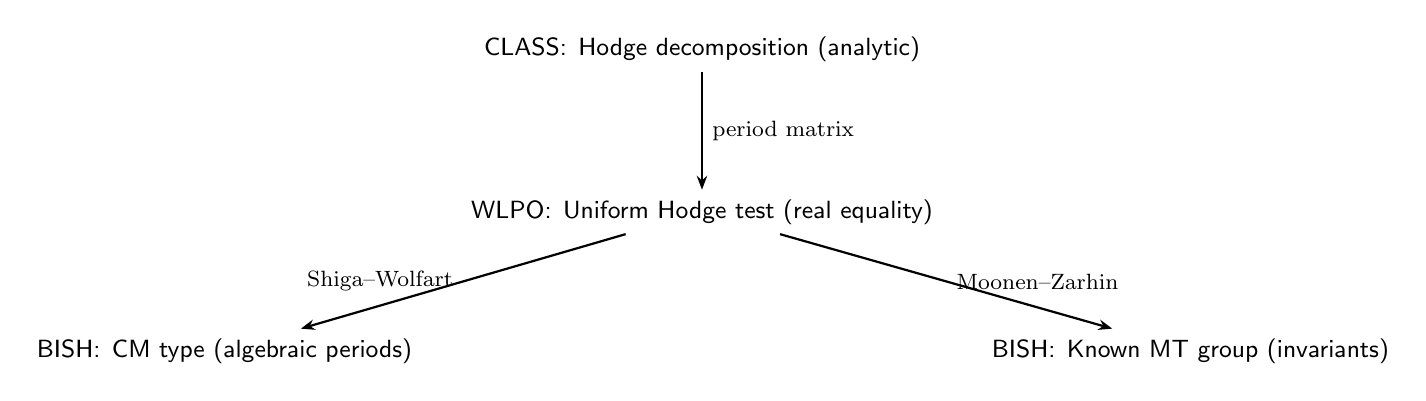
\begin{tikzpicture}[
  node distance=1.5cm,
  level/.style={font=\sffamily\small},
  arrow/.style={-{Stealth[length=5pt]}, thick}
]
\node[level] (class) {$\CLASS$: Hodge decomposition (analytic)};
\node[level, below=of class] (wlpo) {$\WLPO$: Uniform Hodge test (real equality)};
\node[level, below left=1.2cm and 0.5cm of wlpo] (bish1) {$\BISH$: CM type (algebraic periods)};
\node[level, below right=1.2cm and 0.5cm of wlpo] (bish2) {$\BISH$: Known MT group (invariants)};

\draw[arrow] (class) -- node[right, font=\footnotesize] {period matrix} (wlpo);
\draw[arrow] (wlpo) -- node[left, font=\footnotesize] {Shiga--Wolfart} (bish1);
\draw[arrow] (wlpo) -- node[right, font=\footnotesize] {Moonen--Zarhin} (bish2);
\end{tikzpicture}
\end{center}


% ============================================================
\section{Formal Verification}\label{sec:lean}

\subsection{Lean 4 bundle}

The Lean formalisation consists of 602~lines across 6~files, with 0~\texttt{sorry}:

\begin{center}
\begin{tabular}{lr}
\toprule
\textbf{File} & \textbf{Lines} \\
\midrule
\texttt{CRMLevel.lean} --- CRM hierarchy & 56 \\
\texttt{HodgeTest.lean} --- Uniform test, embedding reduction & 148 \\
\texttt{CMDecidable.lean} --- Theorem A, cost function & 116 \\
\texttt{Biconditional.lean} --- Theorem C & 82 \\
\texttt{ShigaWolfart.lean} --- Theorem D & 107 \\
\texttt{Paper87\_HodgeCost.lean} --- Main, axiom inventory & 93 \\
\midrule
\textbf{Total} & \textbf{602} \\
\bottomrule
\end{tabular}
\end{center}

\subsection{Key formalisation: the embedding reduction}

The central proof (Theorem~B, forward direction) in Lean:

\begin{lstlisting}[style=leanstyle]
theorem uniform_hodge_test_implies_wlpo
    (decider : forall (g : Nat) (Omega : AnalyticPeriodMatrix g)
      (idx : Nat), Decidable (is_hodge_analytic Omega idx)) :
    WLPO_Real := by
  intro x
  cases decider 2 (embed_real x) 0 with
  | isTrue h  => left;  rw [<- embed_proj x]; exact h
  | isFalse h => right; intro hx; apply h;
                  rw [<- embed_proj x] at hx; exact hx
\end{lstlisting}

The full equivalence:

\begin{lstlisting}[style=leanstyle]
theorem uniform_hodge_iff_wlpo :
    (forall (g : Nat) (Omega : AnalyticPeriodMatrix g) (idx : Nat),
      (is_hodge_analytic Omega idx) ∨
        ¬(is_hodge_analytic Omega idx))
    <-> WLPO_Real := by
  constructor
  . intro h x
    have := h 2 (embed_real x) 0
    unfold is_hodge_analytic at this
    rw [embed_proj] at this; exact this
  . exact wlpo_implies_uniform_hodge_decidable
\end{lstlisting}

\subsection{Axiom inventory}

\begin{center}
\begin{tabular}{lll}
\toprule
\textbf{Axiom} & \textbf{Type} & \textbf{Justification} \\
\midrule
\multicolumn{3}{l}{\emph{Infrastructure (Lean core)}} \\
\texttt{propext} & Infrastructure & Lean core \\
\texttt{Classical.choice} & Infrastructure & Required for $\R$-valued results \\
\texttt{Quot.sound} & Infrastructure & Lean core \\
\midrule
\multicolumn{3}{l}{\emph{HodgeTest.lean --- Theorem B}} \\
\texttt{AnalyticPeriodMatrix} & Mathematical & Abstract $\Hg$ \\
\texttt{hodge\_projection} & Mathematical & Hodge projection function \\
\texttt{embed\_real} & Mathematical & Period matrix perturbation \\
\texttt{embed\_proj} & Mathematical & Embedding recovers $x$ (Section~\ref{sec:thmB}, Step~3) \\
\midrule
\multicolumn{3}{l}{\emph{CMDecidable.lean --- Theorems A and C}} \\
\texttt{cm\_hodge\_cost} & Mathematical & Opaque CRM cost constant (CM route) \\
\texttt{cm\_hodge\_cost\_eq} & Mathematical & Shiga--Wolfart + $K$-algebra $\Rightarrow \BISH$ \\
\texttt{mt\_hodge\_cost} & Mathematical & Opaque CRM cost constant (MT route) \\
\texttt{mt\_hodge\_cost\_eq} & Mathematical & MT invariants, $\Q$-linear algebra $\Rightarrow \BISH$ \\
\texttt{bare\_hodge\_cost} & Mathematical & Opaque CRM cost constant (bare route) \\
\texttt{bare\_hodge\_cost\_eq} & Mathematical & Bridges--Richman 1987 $\Rightarrow \WLPO$ \\
\midrule
\multicolumn{3}{l}{\emph{ShigaWolfart.lean --- Theorem D}} \\
\texttt{AbelianVarietyOverQbar} & Mathematical & Abstract abelian variety type \\
\texttt{period\_entries\_algebraic} & Mathematical & Algebraic period predicate \\
\texttt{has\_CM} & Mathematical & CM predicate \\
\texttt{shiga\_wolfart} & Mathematical & Shiga--Wolfart 1995 biconditional \\
\texttt{MT\_group} & Mathematical & Abstract Mumford--Tate group type \\
\texttt{ell\_adic\_group} & Mathematical & Abstract $\ell$-adic monodromy group type \\
\texttt{MT\_equals\_Gell} & Mathematical & Mumford--Tate conjecture predicate \\
\texttt{hodge\_classes\_computable\_from\_Gell} & Mathematical & Computability from $G_\ell$ \\
\texttt{mt\_conjecture\_gives\_computability} & Mathematical & MT conjecture $\Rightarrow$ computability \\
\bottomrule
\end{tabular}
\end{center}

The mathematical axioms encode proven theorems from the literature (Shiga--Wolfart, Bridges--Richman, Moonen--Zarhin), not assumptions. The ShigaWolfart.lean axioms serve Theorem~D and the Mumford--Tate conjecture remark; they do not appear in the \texttt{\#print axioms} output of Theorems~A--C. The infrastructure axioms are standard for any Lean~4 formalisation involving~$\R$.

\subsubsection{\texttt{\#print axioms} output}

\begin{lstlisting}[style=leanstyle,numbers=none]
-- uniform_hodge_test_implies_wlpo:
--   propext, Classical.choice, Quot.sound,
--   AnalyticPeriodMatrix, hodge_projection,
--   embed_real, embed_proj

-- hodge_test_biconditional:
--   cm_hodge_cost, cm_hodge_cost_eq,
--   mt_hodge_cost, mt_hodge_cost_eq,
--   bare_hodge_cost, bare_hodge_cost_eq
\end{lstlisting}

Clean separation: Theorem~B depends on the embedding axioms; Theorem~C depends on the cost axioms. No cross-contamination.

\subsection{Reproducibility}

\textbf{Toolchain:} \texttt{leanprover/lean4:v4.29.0-rc2}.
\textbf{Dependency:} Mathlib (fetched automatically by \texttt{lake}).

\begin{verbatim}
cd P87_HodgeCost && lake build
\end{verbatim}

\noindent
\textbf{Zenodo:} \url{https://doi.org/10.5281/zenodo.18809903}

% ============================================================
\section{Discussion}\label{sec:discussion}

\subsection{Relationship to the DPT trilogy}

Paper~87 extends the DPT framework from the Standard Conjectures (Papers~72--74) to the Hodge conjecture. The biconditional structure is identical: $\BISH$-decidability iff algebraic structural condition. The novelty is the target: the Hodge condition is the input to the Millennium Problem, not a stand-alone conjecture.

The $\WLPO$ cost of the uniform Hodge test matches Paper~74's $\WLPO$ cost for eigenvalue comparison. Both involve testing whether a specific real number equals zero: a spectral parameter in Paper~74, a period integral in Paper~87. The common mechanism is $u(\R) = \infty$: the infinite-dimensional nature of $\R$ forces equality testing to be non-constructive.

\subsection{Worked example: Theorem A for $E \times E$ with $\End(E) \cong \Z[i]$}

To make Theorem~A(i) concrete, consider the CM elliptic curve $E: y^2 = x^3 - x$ with $\End(E) \cong \Z[i]$. The abelian surface $A = E \times E$ has CM type $(\Q(i), \{\mathrm{id}, \mathrm{id}\})$. By the Shimura--Taniyama formula, the period matrix is $\Omega_0 = \begin{psmallmatrix} i & 0 \\ 0 & i \end{psmallmatrix}$.

The Hodge decomposition on $H^2(A, \C) \cong \bigwedge^2(\C^4)$ splits into $H^{2,0} \oplus H^{1,1} \oplus H^{0,2}$ with dimensions $1 + 4 + 1 = 6$. A rational class $\alpha \in H^2(A, \Q)$ is Hodge if and only if $\pi_{2,0}(\alpha) = 0$ and $\pi_{0,2}(\alpha) = 0$. For $A = E \times E$:
\begin{itemize}
\item The polarisation class $\omega = e_1 \wedge e_3 + e_2 \wedge e_4$ is a Hodge class. The projections $\pi_{2,0}(\omega)$ and $\pi_{0,2}(\omega)$ vanish identically because $\omega$ generates the Lefschetz ring.
\item The ``diagonal'' class $\delta = e_1 \wedge e_4 - e_2 \wedge e_3$ is also a Hodge class, corresponding to the graph of the CM endomorphism $i \in \End(E)$.
\end{itemize}
The computation of $\pi_{2,0}(\alpha) = 0$ reduces to checking that certain $\Q(i)$-linear combinations of the period entries vanish. Since all entries of $\Omega_0$ lie in $\Q(i)$, this is exact arithmetic: test whether $i \cdot 1 - i \cdot 1 = 0$ (for the polarisation class) or $i \cdot i - (-1) = 0$ (for the CM class). Both are decidable polynomial identity tests over $\Q$, hence $\BISH$.

\subsection{Relationship to the CRMLint Squeeze papers}

Papers~80--85 provided the computational evidence that Theorem~A abstracts. Each Squeeze paper demonstrated $\BISH$-decidability for a specific CM family:
\begin{itemize}
\item Papers~80--83: Gauss--Manin pipeline for the Legendre family (Picard rank computation via Griffiths pole reduction, flat sections, Kovacic maximality).
\item Papers~84--85: Exotic Weil classes on hyperelliptic Jacobians ($\Q(i)$-action, Gauss--Manin block decomposition).
\end{itemize}
In each case, the CM structure algebraises the Hodge-theoretic input, exactly as Theorem~A predicts. Paper~87 identifies the general principle behind these computations.

\subsection{What's next}

The conservation question (Section~\ref{sec:consequences}) is the natural next target. If the Hodge conjecture conserves over $\BISH$, then the CRM program can identify the constructive core of any future proof. If it does not conserve, the failure point would reveal new structural information about the conjecture.

The Mumford--Tate conjecture interface is also promising: a CRM analysis of the MT conjecture itself (is $\MT(A) = G_\ell(A)$ a $\BISH$ statement?) would further clarify the relationship between analytic and algebraic invariants.


% ============================================================
\section{Conclusion}\label{sec:conclusion}

The omniscience cost of the Hodge condition is $\WLPO$ uniformly and $\BISH$ with algebraic metadata. This is the first CRM analysis of a Clay Millennium Problem. It reveals that the difficulty of the Hodge conjecture has two independent sources: the non-constructive cost of \emph{identifying} Hodge classes (measured by this paper) and the unknown cost of \emph{proving algebraicity} (the conjecture itself). All known results operate where the first cost vanishes --- the CM locus and the generic locus --- leaving the algebraicity bridge as the sole remaining challenge.


% ============================================================
\section*{Acknowledgments}

This work was developed with AI assistance (Anthropic Claude, model claude-opus-4-6) for Lean~4 formalisation and manuscript preparation. The mathematical content, proofs, and strategic decisions are the author's. The CRM program is built on the Lean~4 proof assistant and the Mathlib library; the author thanks the Lean and Mathlib communities for their infrastructure.



% ============================================================
\begin{thebibliography}{30}

\bibitem{BridgesRichman1987}
D.~Bridges and F.~Richman,
\textit{Varieties of Constructive Mathematics},
London Mathematical Society Lecture Note Series~97,
Cambridge University Press, 1987.

\bibitem{Cohen1996}
P.~Cohen,
Humbert surfaces and transcendence properties of automorphic functions,
in: \textit{Diophantine Approximation and Abelian Varieties},
Lecture Notes in Mathematics~1566, Springer, 1996.

\bibitem{Deligne1982}
P.~Deligne,
Hodge cycles on abelian varieties,
in: \textit{Hodge Cycles, Motives, and Shimura Varieties},
Lecture Notes in Mathematics~900, Springer, 1982, pp.~9--100.

\bibitem{Grothendieck1969}
A.~Grothendieck,
Standard conjectures on algebraic cycles,
in: \textit{Algebraic Geometry (Bombay 1968)}, Oxford University Press, 1969, pp.~193--199.

\bibitem{Hodge1950}
W.V.D.~Hodge,
The topological invariants of algebraic varieties,
in: \textit{Proceedings of the International Congress of Mathematicians 1950}, vol.~1, pp.~182--192.

\bibitem{Moonen1999}
B.~Moonen,
Notes on Mumford--Tate groups,
preprint, 1999.

\bibitem{MoonenZarhin1999}
B.~Moonen and Yu.~Zarhin,
Hodge classes on abelian varieties of low dimension,
\textit{Mathematische Annalen}, 315 (1999), 711--733.

\bibitem{Shimura1971}
G.~Shimura,
\textit{Introduction to the Arithmetic Theory of Automorphic Functions},
Princeton University Press, 1971.

\bibitem{ShigaWolfart1995}
H.~Shiga and J.~Wolfart,
Criteria for complex multiplication and transcendence properties of automorphic functions,
\textit{Journal f\"ur die reine und angewandte Mathematik}, 463 (1995), 1--25.

\bibitem{Voisin2002}
C.~Voisin,
\textit{Hodge Theory and Complex Algebraic Geometry I--II},
Cambridge Studies in Advanced Mathematics~76--77,
Cambridge University Press, 2002--2003.

\bibitem{Wustholz1989}
G.~W\"ustholz,
Algebraische Punkte auf analytischen Untergruppen algebraischer Gruppen,
\textit{Annals of Mathematics}, 129 (1989), 501--517.

\bibitem{P72}
P.C.K.~Lee,
Characterisation of DPT axioms via constructive reverse mathematics,
Paper~72 of the CRM Series, Zenodo, 2025.
DOI: 10.5281/zenodo.15019571.

\bibitem{P73}
P.C.K.~Lee,
Standard Conjecture~D as a reverse theorem,
Paper~73 of the CRM Series, Zenodo, 2025.
DOI: 10.5281/zenodo.15019579.

\bibitem{P74}
P.C.K.~Lee,
Algebraic spectrum as a reverse theorem,
Paper~74 of the CRM Series, Zenodo, 2025.
DOI: 10.5281/zenodo.15019585.

\bibitem{P80}
P.C.K.~Lee,
Algebraic Gauss--Manin via Griffiths pole reduction over $\Q(t)$,
Paper~80 of the CRM Series, Zenodo, 2026.
DOI: 10.5281/zenodo.18791985.

\bibitem{P81}
P.C.K.~Lee,
Algebraic flat sections and the Theorem of the Fixed Part,
Paper~81 of the CRM Series, Zenodo, 2026.
DOI: 10.5281/zenodo.18801814.

\bibitem{P82}
P.C.K.~Lee,
Constructive differential Galois theory via Kovacic's algorithm,
Paper~82 of the CRM Series, Zenodo, 2026.
DOI: 10.5281/zenodo.18801822.

\bibitem{P83}
P.C.K.~Lee,
Generic Picard number of $E_t \times E_t$,
Paper~83 of the CRM Series, Zenodo, 2026.
DOI: 10.5281/zenodo.18801826.

\bibitem{P84}
P.C.K.~Lee,
Global flatness of Weil classes via Gauss--Manin block decomposition,
Paper~84 of the CRM Series, Zenodo, 2026.
DOI: 10.5281/zenodo.18802819.

\bibitem{P85}
P.C.K.~Lee,
Universal flatness of exotic Weil classes for genus-4 hyperelliptic families,
Paper~85 of the CRM Series, Zenodo, 2026.
DOI: 10.5281/zenodo.18806608.

\bibitem{FormatGuide}
P.C.K.~Lee,
CRM Series Format Guide,
Zenodo, 2025.

\end{thebibliography}

\end{document}
